\documentclass[pdftex,a4paper]{scrreprt}
\usepackage[utf8]{inputenc}       
\usepackage[T1]{fontenc}
\usepackage{graphicx}
\usepackage{xcolor}
\usepackage{booktabs}

\usepackage[
	round,	%(defaultage in the main file and \input ) for round parentheses;
	authoryear,% (default) for author-year citations;
	sort,		% orders multiple citations into the sequence in which they 
]{natbib}	
\usepackage{csvsimple}  % read csv files into Latex


\title{Supplemental Materials for the paper: \\Pesticides pollution of small streams in
Germany}
\author{Eduard Szöcs, Marvin Brinke, Bilgin Karaoglan, Ralf B. Schäfer}

\begin{document}
\maketitle

\chapter{Data Cleaning}
Each of more then 30 datasets have been cleaned and homogenized separately, before combing in a common database.
Cleaning steps comprised (Figure~\ref{fig:data_cleaning} gives a graphical overview).

\begin{enumerate}
	\item Structure: Structure has been adjusted to the database structure.
	\item Coordinates: Coordinates have been transformed to a common Coordinate Reference System (DHDN / 3-Grad Gauss-Krüger Zone 3 (EPSG:31467) and duplicates merged.
	\item Chemicals: Chemical names and identifiers have been unified using the webchem package \citep{szocs_webchem:_2016}.
	\item  Identifiers: Unique identifiers have been assigned.
	\item Units: All concentrations have been converted to $\mu g/L$. Values below limit of quantification have be set to zero.
	\item Other meta-data: meta-data has been standardised.
	\item Temporal resolution: The temporal resolution of the database is 1 day. Date below this resolution has been aggregated by maximum.
	\item Validity Checks: Simple rules for validity checks have been implemented (e.g. no negative concentrations).
\end{enumerate}

\begin{figure}
\centering
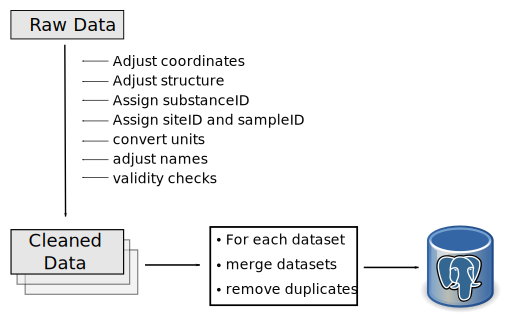
\includegraphics[width = 0.8\textwidth]{data_cleaning}
\caption{Overview on data cleaning steps. After cleaning data has been stored in a relational spatial PostgreSQL database.}
\label{fig:data_cleaning}
\end{figure}

\chapter{Overview on compiled data}

% table generate in do_overview.R
\begin{table}[ht]
\centering
\caption[Overview on chemical samples.]{Overview on chemical samples. Only data from running waters and grab
sampling is shown. \textsuperscript{a}: Abbreviations according to ISO 3166-2:DE. 
      \textsuperscript{b}: Including metabolites} 
\label{tab:phch_overview}
\begin{tabular}{p{2.7cm}lllR{2cm}R{2cm}R{2cm}}
  \toprule
name & abbrv.\textsuperscript{a} & Begin & End & No. sites & No.samples & No. pesticides\textsuperscript{b} \\ 
  \midrule
Baden-Württemberg & BW & 2005-03-10 & 2014-10-02 & 7 & 172 & 98 \\ 
  Bavaria & BY & 2006-04-19 & 2013-12-17 & 13 & 218 & 155 \\ 
  Hesse & HE & 2007-01-15 & 2014-12-18 & 65 & 2411 & 144 \\ 
  Mecklenburg-Western Pomerania & MV & 2005-03-08 & 2014-12-17 & 130 & 1503 & 227 \\ 
  Lower Saxony & NI & 2014-03-24 & 2014-10-13 & 1 & 7 & 226 \\ 
  North Rhine-Westphalia & NW & 2005-01-18 & 2015-01-22 & 1139 & 8536 & 198 \\ 
  Rhineland-Palatinate & RP & 2008-01-02 & 2013-12-18 & 7 & 341 & 236 \\ 
  Schleswig-Holstein & SH & 2005-04-26 & 2014-11-26 & 269 & 1380 & 180 \\ 
  Saarland & SL & 2005-01-03 & 2013-11-25 & 2 & 104 & 57 \\ 
  Saxony & SN & 2005-01-02 & 2013-12-18 & 606 & 9141 & 173 \\ 
  Saxony-Anhalt & ST & 2005-01-24 & 2015-03-19 & 30 & 416 & 88 \\ 
  Thuringia & TH & 2005-06-16 & 2014-12-08 & 32 & 514 & 63 \\ 
   \midrule
 & Total & 2005-01-02 & 2015-03-19 & 2301 & 24743 & 478 \\ 
   \bottomrule
\end{tabular}
\end{table}



\bibliographystyle{apalike}      % basic style, author-year citations
\bibliography{references}

\end{document}